\documentclass[a4paper,11pt, twoside]{article}
\newcommand{\n}[1]{\textbf{#1}}
\usepackage{graphicx}
\usepackage{amsfonts}
\usepackage{amsmath}
\usepackage[brazilian]{babel}
\usepackage[utf8]{inputenc}
\usepackage[T1]{fontenc}
\usepackage {multirow}
\usepackage {booktabs}
\usepackage {fancyhdr}
\usepackage {graphicx}
\usepackage{xcolor}
\linespread {1.5}
\date{\today}
\author{Caio Vinícius Dadauto - 7994808}
\title{Exercicío de Programa 1}
\usepackage{listings}
\lstset{numbers=left,
stepnumber=1,
firstnumber=1,
numberstyle=\tiny,
extendedchars=false,
breaklines=flase,
tabsize=2,
showtabs=true,
tab=\textcolor{gray}{$\cdots$},
frame=tb,
basicstyle=\footnotesize,
stringstyle=\ttfamily,
showstringspaces=false}
\renewcommand{\lstlistingname}{Programa}
\renewcommand{\lstlistlistingname}{Lista de Listagens}
\begin{document}
    \pagestyle{fancy}
    \fancyhf{}
    \renewcommand{\footrulewidth}{0.1pt}
    \renewcommand{\headrulewidth}{0.0pt}
    \fancyfoot[LE, RO]{\bfseries \thepage}

    \begin{center}
        \begin{tabular}{c}
            {\huge Exercício de Programa 1}\\[-0.5cm]
            \rule{0.6\textwidth}{0.1mm}\\
            Caio Vnícius Dadauto$\quad$7994808\\
            {\small 02 de abril de 2013}
        \end{tabular}
    \end{center}
    \vspace{2cm}

    \section*{Problema (a)}
    \subsection*{Análise}
    Tem-se que a função $f(x)$ é dada por:
    \begin{equation}
        f(x) = x^3 - \cos(x^2)
    \end{equation}
    
    Como $0\le \cos (x^2) \le 1$ para $0\leq x\le 1.26$ e, ainda, sabendo que $x^3$ é crescente $\forall x \in\mathbb{R}$,
    pode-se inferir que,
    \begin{equation*}
        0\,<\,\xi\,<\,1.26\,\sim\,\sqrt{\pi / 2}
    \end{equation*}
    onde $\xi$ é a raiz de $f(x)$.
    
    Tendo em vista o método da bisseção para aproximar $\xi$, é possível (a partir da inferencia acima)
    assumir que os pontos iniciais $x_1$ e $x_2$ podem assumir o valor de 0 e 1.26, respectivamente.
    Uma vez, que $f(x_1)f(x_2)<0$ o que satisfaz a hipótese inicial para o método da bisseção.
    
    Estimado os valores iniciais de $x_1$ e $x_2$, é possível implementar o seguinte código para
    aproximar $\xi$ através do método da bisseção.\\[0.15cm]
    {\linespread{1.15}
    \lstinputlisting[language=C, label=sqlselect, caption={Implementação para o método da bisseção.}]{bi.c}}
    
    \subsection*{Resultados}
    Após ter executado o programa, obteve-se os resultados apresentados na tabela \ref{bi}.
    	{\linespread{1}
	\begin{table}[!th]
		\begin{center}
		    \begin{tabular}{ c c c c c c c }
		        \toprule[0.11em]
		        \n{Interação (k)} & \n{$x_1$} & \n{$x_2$} & \n{$x_m$} & \n{$f(x_1)$} & \n{$f(x_2)$} & \n{$f(x_m)$}\\
		        \toprule[0.11em]
				1 & 0.0000 & 1.2600 & 0.6300 & -1.0000 & 2.0172 & -0.6722\\
				\midrule
				2 & 0.6300 & 1.2600 & 0.9450 & -0.6722 & 2.0172 & 0.2169\\
				\midrule
				3 & 0.6300 & 0.9450 & 0.7875 & -0.6722 & 0.2169 & -0.3254\\
				\midrule
				4 & 0.7875 & 0.9450 & 0.8663 & -0.3254 & 0.2169 & -0.0814\\
				\midrule
				5 & 0.8663 & 0.9450 & 0.9056 & -0.0814 & 0.2169 & 0.0606\\
				\midrule
				6 & 0.8663 & 0.9056 & 0.8859 & -0.0814 & 0.0606 & -0.0121\\
				\midrule
				7 & 0.8859 & 0.9056 & 0.8958 & -0.0121 & 0.0606 & 0.0238\\
				\midrule
				8 & 0.8859 & 0.8958 & 0.8909 & -0.0121 & 0.0238 & 0.0058\\
				\midrule
				9 & 0.8859 & 0.8909 & 0.8884 & -0.0121 & 0.0058 & -0.0032\\
				\midrule
				10 & 0.8884 & 0.8909 & 0.8896 & -0.0032 & 0.0058 & 0.0013\\
				\midrule
				11 & 0.8884 & 0.8896 & 0.8890 & -0.0032 & 0.0013 & -0.0010\\
				\midrule
				12 & 0.8890 & 0.8896 & 0.8893 & -0.0010 & 0.0013 & 0.0001\\
				\midrule
				13 & 0.8890 & 0.8893 & 0.8892 & -0.0010 & 0.0001 & -0.0004\\
				\midrule
				14 & 0.8892 & 0.8893 & 0.8892 & -0.0004 & 0.0001 & -0.0001\\
		        \toprule[0.11em]
		        \multicolumn{7}{c}{\n{Raiz ($\xi$)}}\\
		        \toprule[0.11em]
		        \multicolumn{7}{c}{0.8892}\\
		        \midrule
		    \end{tabular}
		\end{center}
		\caption{Resultados obtidos no método da bissecão.\label{bi}}
	\end{table}}
	
	Tem-se que a derivada de $f(x)$ é:
	\begin{equation}
	    f'(x) = 3x^2 + 2x\sin(x^2)
	\end{equation}
	
    A partir da derivada, pode-se inferir que $f'(x)>0$ para $x\geq -2/3$.
    Assim, pelo teorema do valor médio, tem-se que $f(x)$ é crescente para $x\geq -2/3$.
    Como $f(-2/3)<0$ e  $f(x)>0$ para algum $x$ maior que $-2/3$, por exemplo $x=1,6$,
    $f(x)$ possui somente uma raiz real para $x\geq -2/3$.
    Por outro lado, $f(x)<0$ para $x<-2/3$, o que implica que $f(x)$ não possui raiz real para $x<-2/3$.
    Logo $f(x)$ possui somente uma raiz real.
    
    \section*{Problema (b)}
    \subsection*{Análise}
    Para estimar a mesma raiz $(\xi)$ de $f(x)$ pelo método de
    Newton-Raphson é necessário que
    \begin{eqnarray}
        \varphi'(c)<1 & \quad\mathrm{para}\;x_k<c<\xi\\
        f'(x_k)\neq 0
    \end{eqnarray}
    onde $x_k$ é
    o valor da variavel livre de $f(x)$ na k-ésima interação e \mbox{$\varphi(x) = x - \frac{f(x)}{f'(x)}$}.
    
    Derivando $f'(x)$, obtem-se que:
    \begin{equation}
        f''(x) = 6x + 2\sin(x^2) + 4x^2\cos(x^2)
    \end{equation}
    
    Como $0\le 2\sin(x^2) + 4x^2\cos(x^2)\le 2$ para $0 \le x \le \pi/2$ é possível inferir que
    $f''(x) > 0$ para $0 \le x \le \pi/2$.
    Logo, tem-se que, pelo teorema do valor médio,
    $f'(x)$ é crescente para $0 \le x \le \pi/2$. Assim, para $0 \le x \le \pi/2$, $f'(x)$ possui apenas a raiz trivial $x=0$.
    Somente o intervalo $0 \le x \le \pi/2$ é considerado, pois sabe-se que $\xi\sim0.89$.
    
    Sendo $\varphi(x)$ dado por,
    \begin{equation}
        \varphi(x) = x - \frac{(x^3 - \cos(x^2))}{3x^2 + 2x\sin(x^2)}
    \end{equation}
    tem-se que sua derivada é dada por,
    \begin{equation}
        \varphi'(x) = \frac{(6x + 2\sin(x^2) + 4x^2\cos(x^2))(x^3 - \cos(x^2))}{{(3x^2 + 2x\sin(x^2))}^2}
    \end{equation}
    como, para o método de Newton-Raphson, $\varphi(c)<1$, tem-se que,
    \begin{eqnarray}
        \varphi'(x) = \frac{(6x + 2\sin(x^2) + 4x^2\cos(x^2))(x^3 - \cos(x^2))}{{(3x^2 + 2x\sin(x^2))}^2} < 1\\
        4x^5\cos(x^2) - (6x\cos(x^2) + 10x^3\sin(x^2) + \sin(2x^2) + 3x^4 + 4x^2) < 0 \label{eq}
    \end{eqnarray}
    
    A partir da equação \eqref{eq} é possível concluir que $\varphi'(x)<1$ para $0 < x \le 1$. Pois, $4x^5\cos(x^2) < 6x\cos(x^2)$
    para $0 < x \le 1$.
    
    Assim, é possível tomar como ponto inicial (x) para a execução do método de Newton-Raphson o valor de 1.
    O código para estimar $\xi$ pelo método de Newton-Raphson é apresentado logo abaixo.\\[0.15cm]
    
    {\linespread{1.15}
    \lstinputlisting[language=C, label=sqlselect, caption={Implementação para o método da Newton-Raphson.}]{new.c}}
    
    \subsection*{Resultados}
    Após ter executado o programa, obteve-se os resultados apresentados na tabela \ref{new}.
    {\linespread{1}
	\begin{table}[!th]
		\begin{center}
		    \begin{tabular}{ c c c c }
		        \toprule[0.11em]
		        \n{Interação (k)} & \n{$x_k$} & \n{$f(x_k)$} & \n{$f'(x_k)$}\\
		        \toprule[0.11em]
			1 & 0.9018 & 0.0464 & 3.7504\\
			\midrule
			2 & 0.8895 & 0.0007 & 3.6386\\
			\midrule
			3 & 0.8893 & 0.0000 & 3.6369\\
		        \toprule[0.11em]
		        \multicolumn{4}{c}{\n{Raiz ($\xi$)}}\\
		        \toprule[0.11em]
		        \multicolumn{4}{c}{0.8893}\\
		        \midrule
		    \end{tabular}
		\end{center}
		\caption{Resultados obtidos no método da Newton-Raphson.\label{new}}
	\end{table}}
	
	\section*{Problema (c)}
	\subsection*{Análise}
	Assume-se que o potêncial de interação em função da distância (r)
	entre os íons de uma molécula diatômica é dado
	por:
	\begin{equation}\label{pot}
	    V(r) = -\frac{e^2}{4\pi\epsilon_0 r} + V_0\exp{(-r / r_0)}
	\end{equation}
	onde $\epsilon_0$ é a permissividade do vácuo,  $e$ é a caraga do elétron e $V_0$ e $r_0$ são
	parâmetros de ação efetiva.
	
	Usando os parâmetros cristalinos ($V_0 = 1.38\cdot10^3$eV e $r_0 = 0.328$\AA) e assumindo
	que $\frac{e^2}{4\pi\epsilon_0} = 14.4$V\AA, é possível plotar o gráfico da funçãoo \eqref{pot}.
	O qual é apresentado na figura \ref{graf-pot}.
	\begin{figure}[!ht]
        \begin{center}
            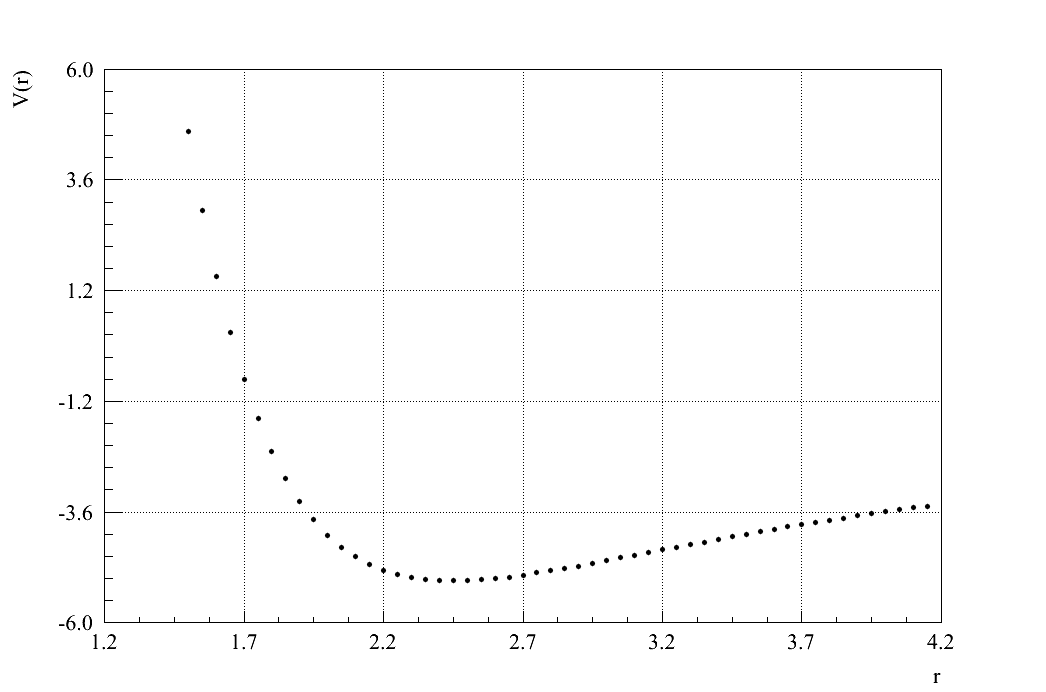
\includegraphics[scale=0.35]{funcao.png}
        \end{center}
        \caption{Gráfico da V(r) por r.\label{graf-pot}}
    \end{figure}
    
    Sabendo que a força que atua entre os átomos é dada por:
    \begin{equation}\label{forca}
        F(r) = -\frac{\mathrm{d}V(r)}{\mathrm{d}r} = -\frac{e^2}{4\pi\epsilon_0 r^2} + \frac{V_0}{r_0}\exp{(-r / r_0)}
    \end{equation}
    
    Plotando o gráfico dado pela função \eqref{forca}, obtem-se o seguinte conjunto de pontos.
	\begin{figure}[!ht]
        \begin{center}
            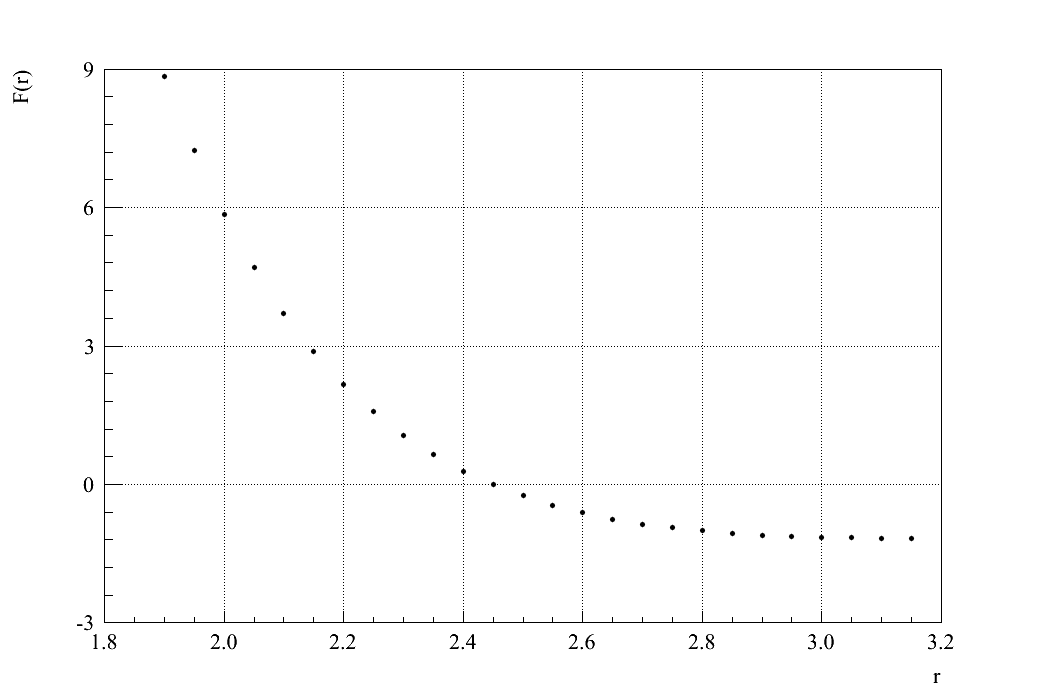
\includegraphics[scale=0.35]{derivada.png}
        \end{center}
        \caption{Gráfico da F(r) por r.\label{graf-forca}}
    \end{figure}
    
    Para que os átomos estejam em equilíbrio e ainda interagindo entra si é necessario que estes estejam espaçados
    de uma distância ($r_{eq}$) que equivale ao ponto de mínimo da função $V(r)$,
    o que implica que $F(r) = 0$.
    
    Tendo como objetivo estimar a distância ($r_{eq}$) através do método das secantes e analisando o
    gráfico da figura \ref{graf-forca} é possível adotar os valores de 2 e 3 para os pontos iniciais $x_1$ e $x_2$, respectivamente.
    Pois é facilmente perceptivel que a raiz de $F(r)$ está no intervalo $2<r<3$ de forma a minimizar $V(r)$.
    
    Novamente analizando o gráfico da figura \ref{graf-forca} é possível inferir que a derivada de $F(r)$ não é zero dentro do intervalo
    $2<r<3$. Pois, a reta tangente ao gráfico da figura \ref{graf-forca} não é paralela a abscissa dentro do intervalo  $2<r<3$.
	
	Assim, implementou-se o código para estimar $r_{eq}$ através do método das secantes.
	Código que segue logo abaixo.
	
	{\linespread{1.15}
    \lstinputlisting[language=C, label=sqlselect, caption={Implementação para o método das secantes.}]{sec.c}}
    
    \subsection*{Resultados}
    Após ter executado o programa, obteve-se os resultados apresentados na tabela \ref{sec}.
    {\linespread{1}
	\begin{table}[!th]
		\begin{center}
		    \begin{tabular}{ c c c }
		        \toprule[0.11em]
		        \n{Interação (k)} & \n{$x_k$} & \n{$F(x_k)$}}\\
		        \toprule[0.11em]
				1 & 2.8358 & -1.0506\\
				\midrule
				2 & 2.7087 & -0.8724\\
				\midrule
				3 & 2.0866 & 3.9568\\
				\midrule
				4 & 2.5963 & -0.6005\\
				\midrule
				5 & 2.5291 & -0.3665\\
				\midrule
				6 & 2.4240 & 0.1465\\
				\midrule
				7 & 2.4540 & -0.0212\\
				\midrule
				8 & 2.4502 & -0.0010\\
				\midrule
				9 & 2.4500 & 0.0000\\
		        \toprule[0.11em]
		        \multicolumn{3}{c}{\n{Raiz (r_{eq})}}\\
		        \toprule[0.11em]
		        \multicolumn{3}{c}{2.4500}\\
		        \midrule
		    \end{tabular}
		\end{center}
		\caption{Resultados obtidos no método das secantes.\label{sec}}
	\end{table}}
\end{document}